	\documentclass[11pt, oneside]{article}   	% use "amsart" instead of "article" for AMSLaTeX format
	\usepackage{geometry}                		% See geometry.pdf to learn the layout options. There are lots.
	\geometry{letterpaper}                   		% ... or a4paper or a5paper or ... 
	%\geometry{landscape}                		% Activate for rotated page geometry
	%\usepackage[parfill]{parskip}    		% Activate to begin paragraphs with an empty line rather than an indent
	\usepackage{graphicx}				% Use pdf, png, jpg, or eps§ with pdflatex; use eps in DVI mode
									% TeX will automatically convert eps --> pdf in pdflatex		
	\usepackage{amssymb}
	
	\usepackage{hyperref}
	\usepackage{caption}
	
	%SetFonts
	
	%SetFonts
	\graphicspath{{images/}}  	% Images folder
	
	\title{Network Analysis of Emails Sent Within Enron}
	\author{Frank Acquaye}
	%\date{}							% Activate to display a given date or no date
	
	\begin{document}
	\maketitle
	
	\section{Network Summary}
	\subsection{Data Source}
	I wanted to explore the network structure of emails sent within \href{https://en.wikipedia.org/wiki/Enron}{Enron}. I used preprocessed data from  \href{http://snap.stanford.edu/data/email-Enron.html}{SNAP}.
	\subsection{Summary Statistics of Enron Emails}
	\emph{Table 1} shows the summary statistics of Enron Emails Network. \\
	\\
	\emph{Figure 1} shows degree distribution \\
	\emph{Figure 2} shows a visualisation of the network using the Force Atlas 2 Algorithm. \\
	\emph{Figure 3} shows a visualisation of the network using the Force Atlas 2 Algorithm with node and edge colouring. \\
	\emph{Figure 4} shows a visualisation of the network using the Yifan Hu Algorithm. \\
	\emph{Figure 5} shows a visualisation of the network communities. \\
	\emph{Figure 6} shows a visualisation of the network communities according to the first 250 nodes of the network according to the page-rank algorithm.\\
	\\
	\par
	Upon inspection one realises a huge cluster within the centre of all visualisations and less connections in the extremities. It's my perception that these clusters are mostly key stakeholders in Enron and perhaps top management within Enron. Since the data used was not labelled this might be a bit hard to confirm.
	\begin{center}
 \begin{tabular}{||p{12cm}||p{5cm}|}
\hline 
\textbf{Statistic Name} & \textbf{Value} \\ \hline
 \textbf{Nodes/Order} & 36692  \\  
 \hline
 \textbf{Edges/Sizer} & 183831  \\  
 \hline
 \textbf{Max Degree} & 1383\\  
 \hline
 \textbf{Min Degree} & 1\\  
 \hline
 \textbf{Mean Degree} & 10.020\\  
 \hline
 \textbf{Number of Connected Components} & 1065\\  
 \hline
  \textbf{Radius} & 7\\  
 \hline
 \textbf{Diameter} & 13\\  
 \hline
 \textbf{Clustering Co-efficient} & 0.497\\  
 \hline
 \hline
 \textbf{Order of largest connected component} & 33696\\  
 \hline
 \textbf{Size of largest connected component} & 180811\\  
 \hline
 \textbf{Ratio of Size of entire Graph to Connected Component} & 0.983\\  
 \hline
 \textbf{Ratio of Order of entire Graph to Connected Component} & 0.918\\  
 \hline
 \textbf{Total Number of traingles} & 727044.0\\  
 \hline
\end{tabular}
\captionof{table}{Summary Statistics for Enron Emails Network}\label{summarystats}

\begin{figure}
  \centering
  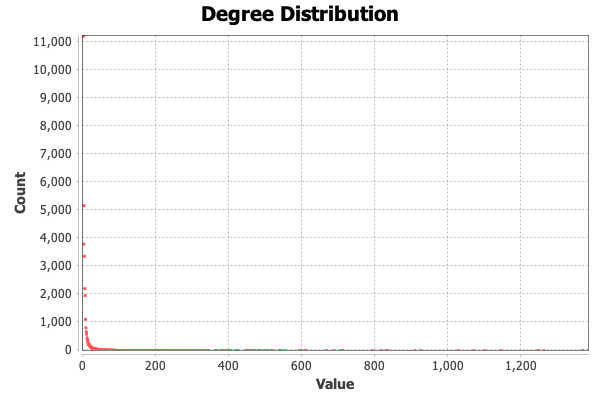
\includegraphics[width=\columnwidth]{degree-distribution.png}
  \caption{Degree Distribbution }
\end{figure}

\end{center} 
		\begin{figure}
  \centering
  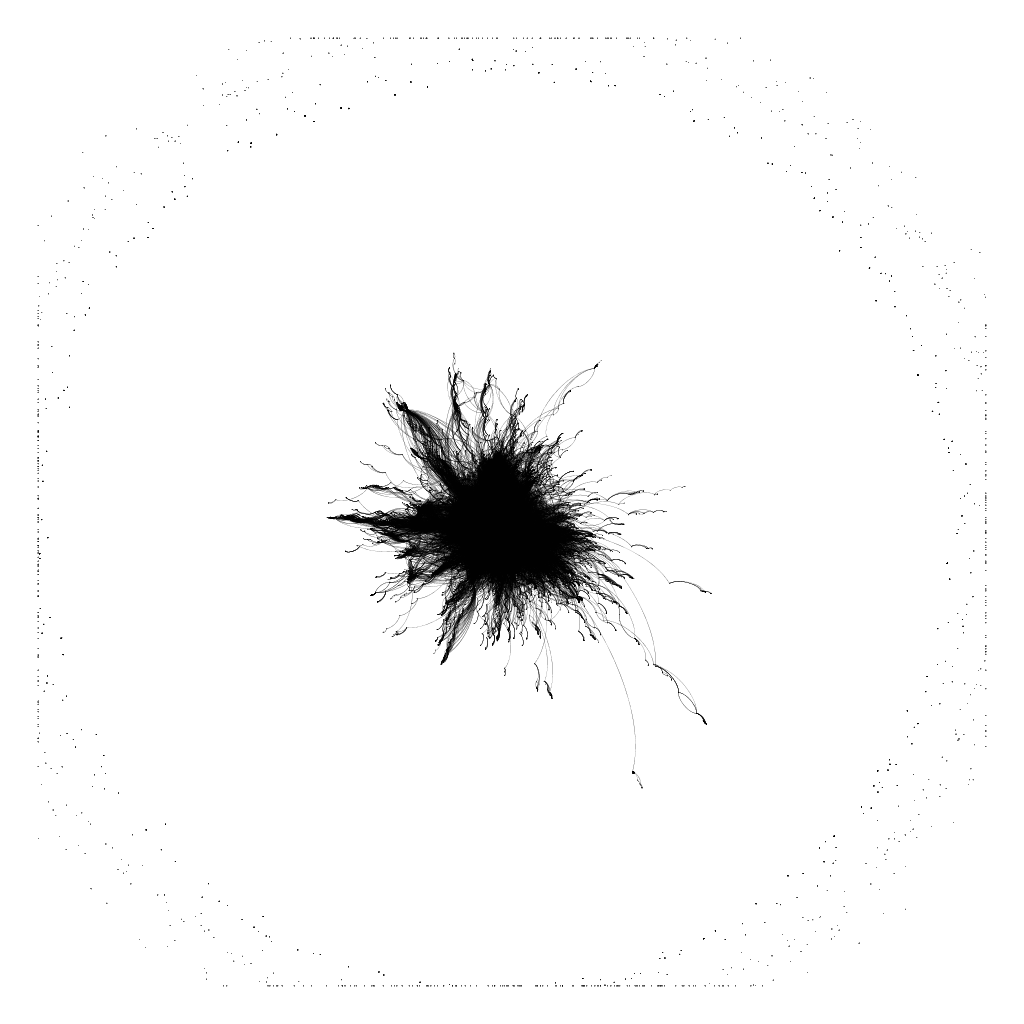
\includegraphics[width=\columnwidth]{enron-force-atlas-2.png}
  \caption{Network Structure of Enron Emails using Force Atlas 2 }
\end{figure}
\begin{figure}
  \centering
  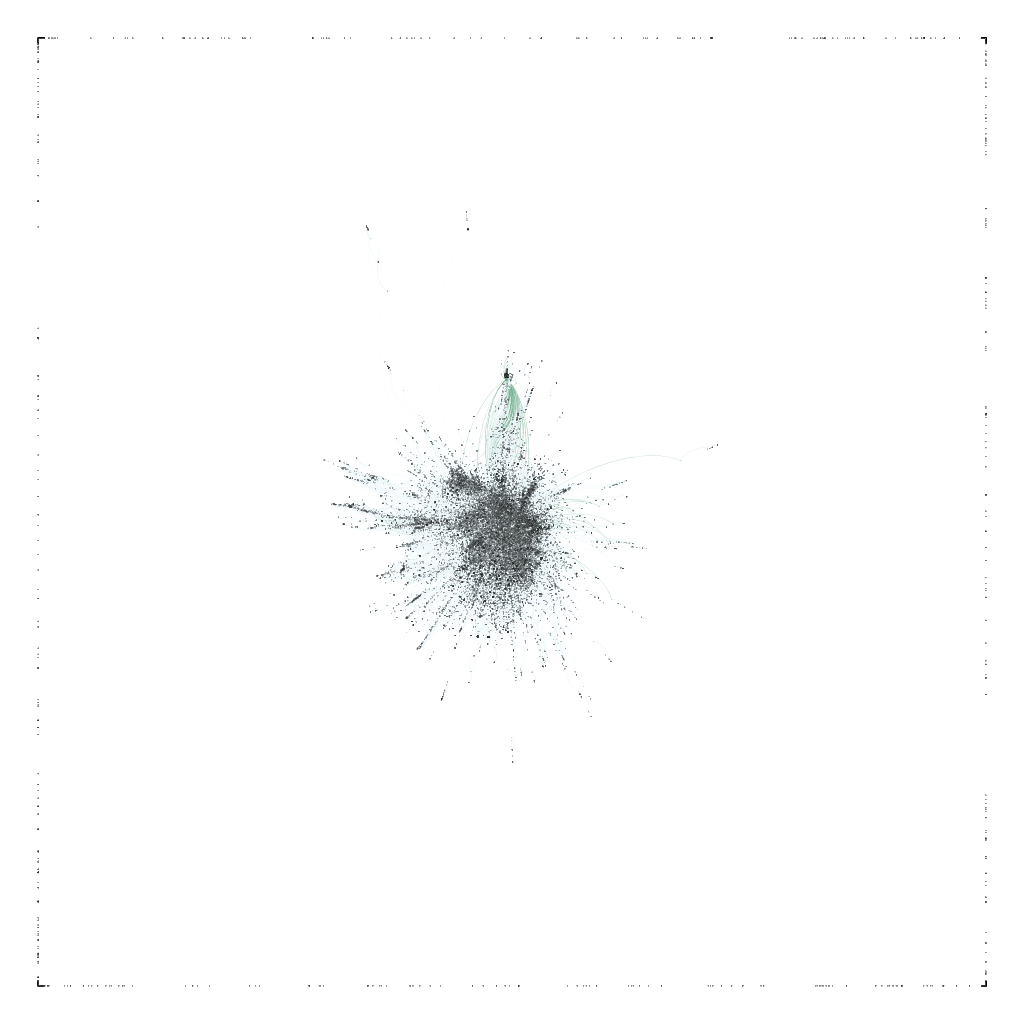
\includegraphics[width=\columnwidth]{enron-graphs.png}
  \caption{Network Structure of Enron Emails using Force Atlas 2  with colouring}
\end{figure}

	\begin{figure}
  \centering
  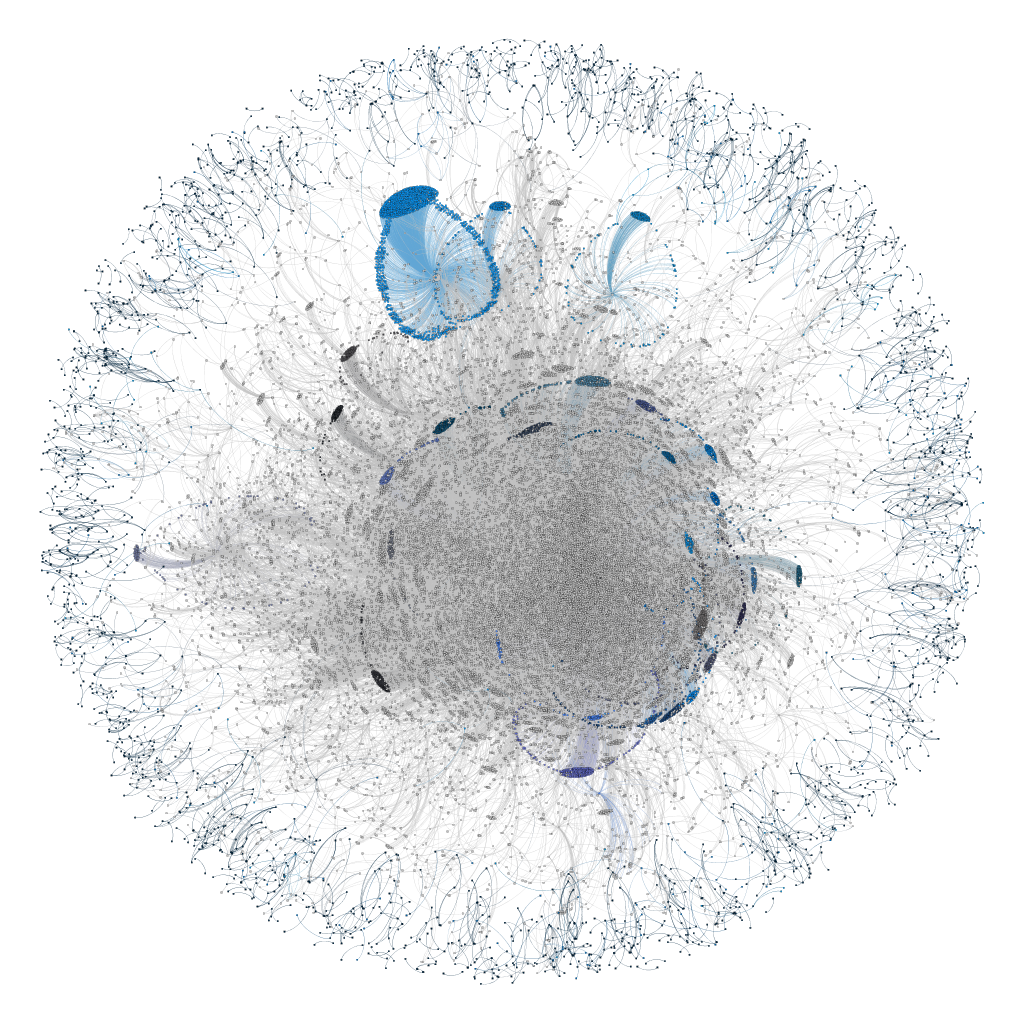
\includegraphics[width=\columnwidth]{na-ee-graph-final.png}
  \caption{Network Structure of Enron Emails using Yifan Hu }
\end{figure}

\pagebreak

\section{Network Structure}
Owing to the huge nature of the network most network, the assortative matrix was computed using a subgraph obtained from the first 250 nodes of the network according to the page-rank algorithm.

\pagebreak

\section{Community Detection}
The image in \emph{Figure 5} is  incomprehensible hence I used the first 250 nodes of the network according to the page-rank algorithm.
\begin{figure}
  \centering
  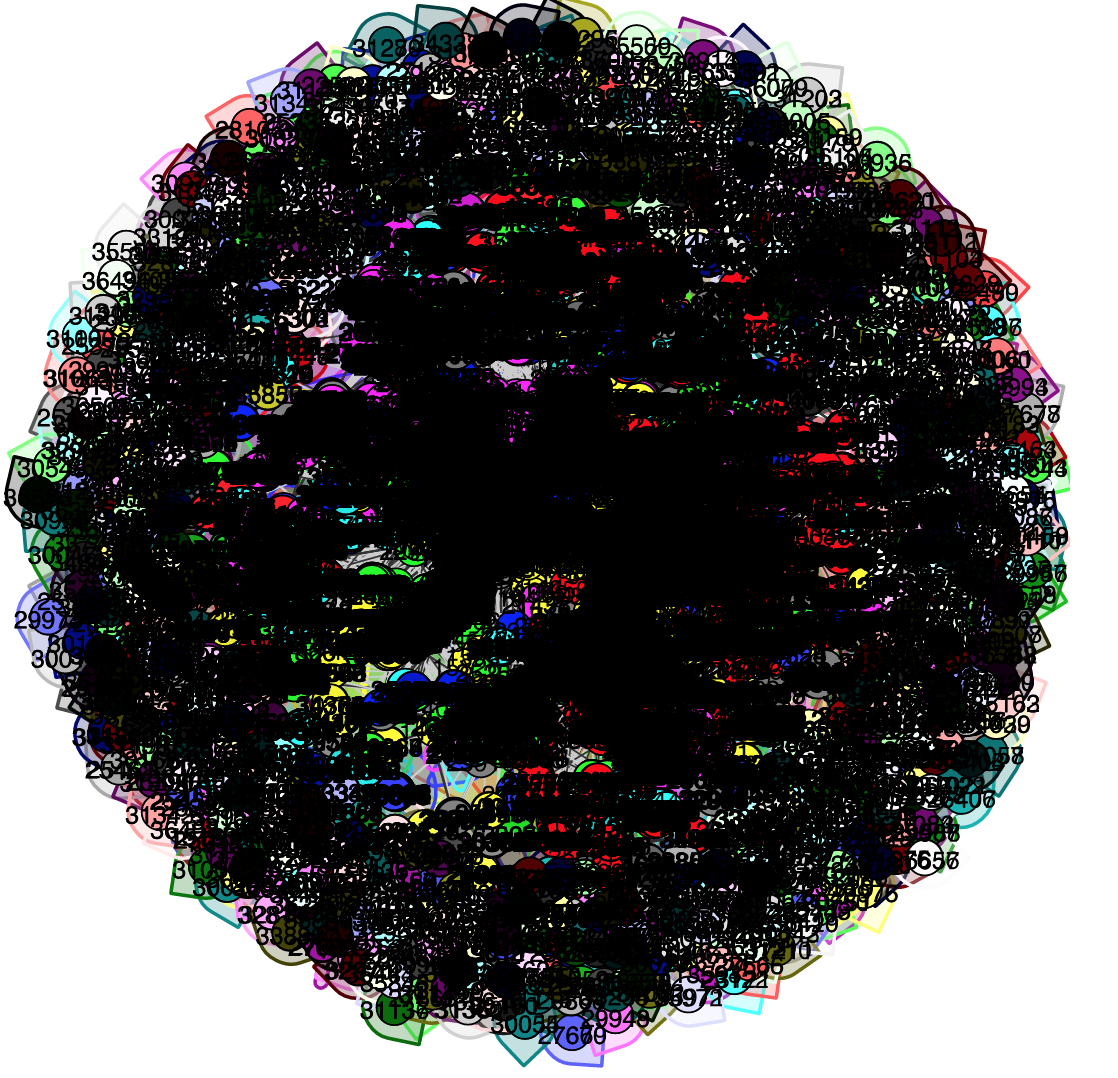
\includegraphics[width=\columnwidth]{communities.png}
  \caption{ Communities in Enron Emails Network}
\end{figure}

\begin{figure}
  \centering
  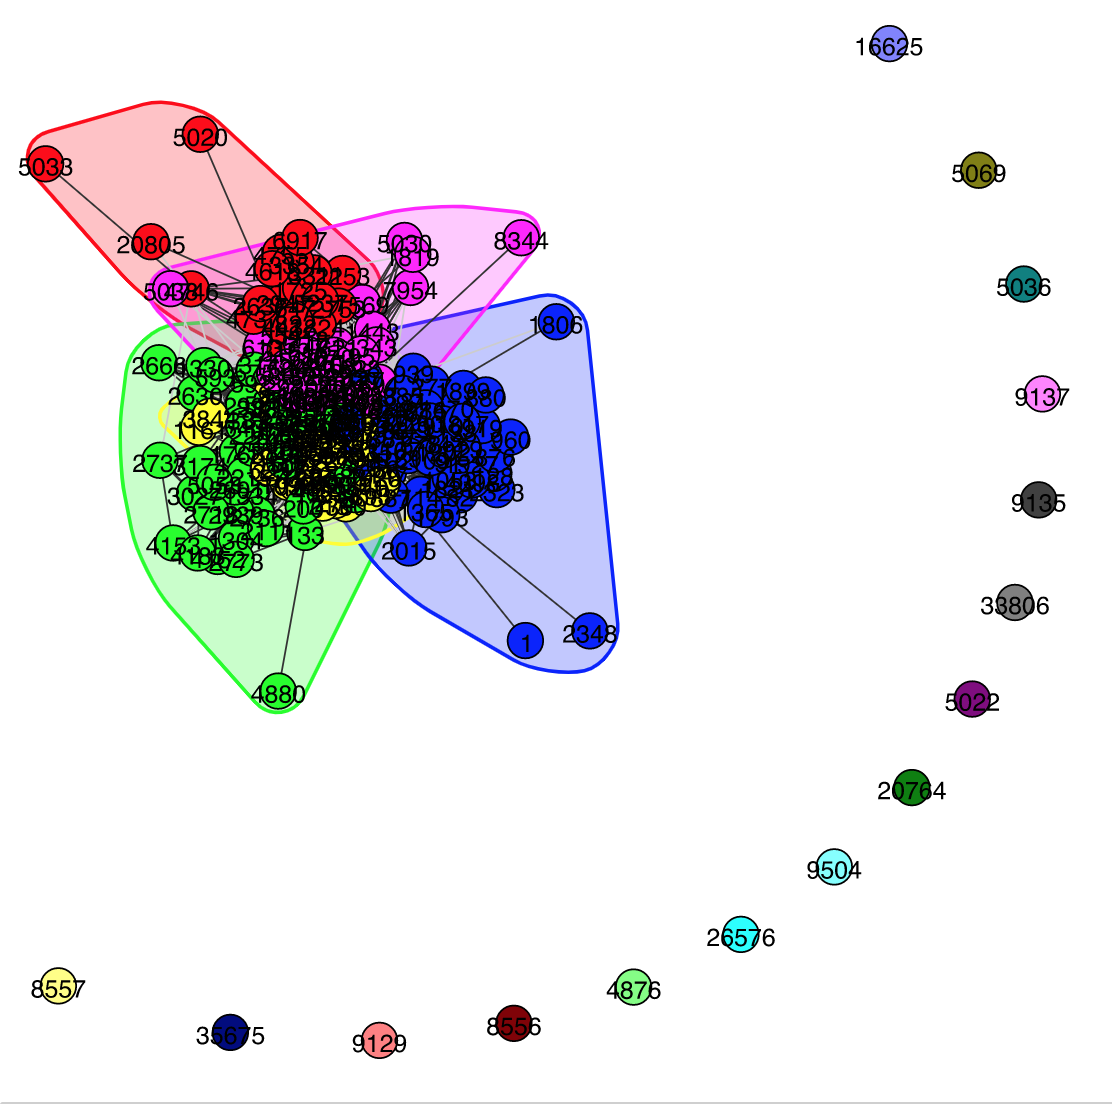
\includegraphics[width=\columnwidth]{communities-page-rank.png}
  \caption{ Communities in Top 250 Enron Emails Network According to Page Rank}
\end{figure}


\end{document}  